\chapter{Processing and Methodologies}
In this chapter, I will introduce the procedure of extracting facial features and the tools and methodologies I use.
\section{Processing Flow}
\paragraph{Processing Chart}
\begin{figure}[ht]
\centering
\includegraphics[width=\textwidth]{imgs/ProcedureChart.png}
\caption{Main Procedure}
\label{fig:proc}
\end{figure}
Figure \ref{fig:proc} shows main procedure of the whole project. At beginning, I tried several trackers. Intraface and DRMF are two trackers I tried and compared most. Two trackers are using different methods and also implemented in different languages. Intraface are programmed in c and matlab and has great interface for matlab. I tried two version of DRMF, DRMF programmed using CUDA which uses parallel processing is quite fast. As the programme of DRMF doesn't integrate extract frames from videos. The images are extracted using external function, then tracked using DRMF. I choose Intraface as the final choose, the reason and comparison will be given in later section. Remove head-pose seems to be a very important part for this project, as subject's head moves frequently in many videos. After having tracking points without head-pose, each face in each frame is warped and scaled to same size grey image. Extracting features is to extract appearance feature of each face in the image. Post-processing is preprocessing before using the data for classification.
\paragraph{Data flow Chart}
\begin{figure}[ht]
\centering
\includegraphics[width=\textwidth]{imgs/DataFlowChart.png}
\caption{Data Flow}
\label{fig:DF}
\end{figure}
Figure \ref{fig:DF} show data I need for processing. There are two types of encoded video, one is in format of fly and the other is avi. Extracting frames from videos is proceed with Intraface and stored in formats of jpeg and mat which used for processing of matlab. There are several situations that a track is unable to track a face in the image such as no subject in the image, the head is face to a very large angle from frontal face, face is partially not show in the frame. Frame index points to those images which the tracker is able to tracker a face in a frame. Image is the frame images stored in mat format. Different tracker may tracks different number of characteristic facial points. Intraface tracks 49 facial points and DRMF tracks 66 points. Deformed points is the tracking point after removed head-pose. Warped Images is the face after remove head-pose and background which only leaves the meshes build by tracking points. Appearance feature is face feature extracted using local binary pattern (LBP). As the image size from image to warped images are changed, the points is rescaled from deformed point to scaled points.

\section{Face Alignment}

Face alignment is to align face in one image with respect to the same face in another image. Face alignment techniques are used to track characteristic facial points in image sequences. In this project, the aim of face alignment is to localise the feature points on face images. The points are usually around eyes, nose, mouth, and outline. Face alignment techniques are essential on face recognition, modelling and synthesis. There are three main different approaches Parametrized Appearance Models(PAMs), Discriminative approaches, Part-based deformable models. Parametrized appearance models contains many models such as active appearance models (AAMs), morphrable models, eigentrackings, and template tracking \cite{xiong2013supervised}. All these models are using PCA method to parametrize a face. A face could approximately decomposed as linear combination of shape basis and appearance basis. The problem of face alignment could be refer as minimising the difference between the constructed PAM and the face. Common approach is use Gauss-Newton methods \cite{xiong2013supervised}. Discriminative approaches are to learn the linear regression between the head move and appearance change. Part-based deformable model perform face alignment by maximising the posterior likelihood of part locations given image\cite{xiong2013supervised}.

\subsection{Active Appearance Model}
Active Appearance Model (AAMs) is defined as a generative model of a certain visual phenomenon in \cite{matthews2004active}. AAMs are conceptually related to morphable models, constrained models and active blobs. In this project, it is refer to a model of face. As AAM is conceptually related to other parameterized appearance model, so it is introduced as an example of parameterized appearance model for understanding purpose. According to \cite{matthews2004active}, there are two types of AAMs, one refers as independent shape and appearance models, which model shape and appearance independently, and the other refers as combined shape and appearance models, which parameterized shape and appearance model with a single set of linear parameters \cite{matthews2004active}. Normally AAMs appears along with a fitting algorithm. However, in the following context, it only refers to a model.\cite{matthews2004active} gave a well explain about what is an AAM, most of following theory are from \cite{matthews2004active}.
\paragraph{Shape}
Shape of a face $s$ is defined by coordinates $(x,y)$ of $v$ vertices of face points and the mesh they built:
\begin{equation}
s = (x_{1},y_{1},x_{2},y_{2},...,x_{v},y_{v})^{T}
\end{equation}
\newline
$s$ also can be expressed as a base shape $s_{0}$ plus linear combination of $n$ shape vectors $s_{i}$:
\begin{equation}
s = s_{i} + \sum_{i =1}^{n}p_{i}s_{i}
\end{equation}
\paragraph{Appearance}
For all pixels x in the mesh $s_{0}$, appearance $A(0)$ can be expressed by base appearance $A_{0}(x)$ and m appearance images $A_{i}(x)$.
\begin{equation}
A(x) = A_{0}(x) + \sum_{i=1}^{m}\lambda_{i}A_{i}(x) \qquad \forall x \in s_{0}
\end{equation}
\newline
AAMs are usually computed by applying Principle Component Analysis (PCA) to choose images. The chosen images contains a variety of shapes. The base shape $s_{0}$ is the mean shape and the vector $s_{v}$ is the eigenvector corresponding to the largest $v$ eigenvalues. The base appearance $A_{0}$ and the appearance $A_{i}$ is computed by applying Principle Component Analysis to a set of shape normalised images.
\paragraph{Model} 
$W(x:p)$ is the warp from $s_{0}$ to $s$. Then the model $M$ set the appearance of $W(x:p)$ to $A(x)$.
\begin{equation}
M(W(x:p)) = A(x)
\end{equation}
\newline
Combined AAMs
\newline
Combined AAMs just use parameter $c = (c_{1},c_{2},...)^{T}$ to parametrize shape:
\begin{equation}
s = s_{0} + \sum_{i=1}^{l}c_{i}s_{i}
\end{equation}
and appearance:
\begin{equation}
A(x) = A_{0}(x) + \sum_{i=1}^{l}c_{i}A_{i}(x)
\end{equation}

\subsection{Trackers}
There are many different trackers for tracking facial feature points. Different tracker may use different approaches, so they may be applied into different situations. I tried two main trackers for tracking characteristic facial points, one is Intraface \cite{xiong2013supervised} which use suppervised decent method, the other is DRMF \cite{asthana2013robust} which use discriminative response map fitting. Those two trackers not only using different approaches, the number of landmark points are also different.
\paragraph{Intraface}
\cite{xiong2013supervised} implies image alignment  can be posed as solving a nonlinear optimization problem. It uses Supervised Descent Method for minimising Non-linear Least Square(NLS) function, which avoids calculating the Hessian and the Jacobian that could be computationally expensive. The running time of Intraface shows that the method is very effective and efficient.
\paragraph{Tracking Points}
The following tracker show the tracking points of Intraface. This tracker tracks 49 facial feature points. As you can see the eyes, nose, mouth, unfortunately the jaw and cheek may contain visual information that would help classification. Without the bound of face, I am unable to extract the region  as I can not do warping of that area.
%insert a figure of tracking face points by intraface.
\paragraph{Eating and Talking Sequence}
Figure \ref{fig:IES} show a sequence of image of eating tracked by Intraface. The point are aligned very precisely along the face. Figure \ref{fig:ITS} shows a talking sequences of image tracked by Intraface. The landmark points of mouth is very accurate.
\begin{figure}[p]
\centering
\includegraphics[width=110mm]{imgs/Tracking_Intraface_eating_red.png}
\caption{Eating sequence tracked by Intraface}
\label{fig:IES}
\includegraphics[width=110mm]{imgs/Talking_Intraface_140711_176_184.png}
\caption{Talking sequence tracked by Intraface}
\label{fig:ITS}
\end{figure}
\newpage
\paragraph{DRMF}
DRMF uses novel discriminative regression based on Constrained Local Models(CLMs) for face alignment. The basic idea of DRMF is to fit a face for each frame of a video. After locating the position of a face, the tracker tries to fit a trained constrained local model to fit the face. Sometimes the fitting result is not very good and the landmark points of mouth region is not very accurate.
\paragraph{Tracking Points}
DRMF tracked 66 facial feature points, the extra 17 points are the point around face bound. Other landmark points are the same with Intraface.
% insert a image of tracking points of face
\paragraph{Talking and Talking Sequence}
A image sequences of eating tracked by Intraface is shown below.
\begin{figure}[p]
\centering
\includegraphics[width=100mm]{imgs/Tracking_DRMF_eating.png}
\caption{Eating sequence tracked by DRMF}
\label{fig:DES}
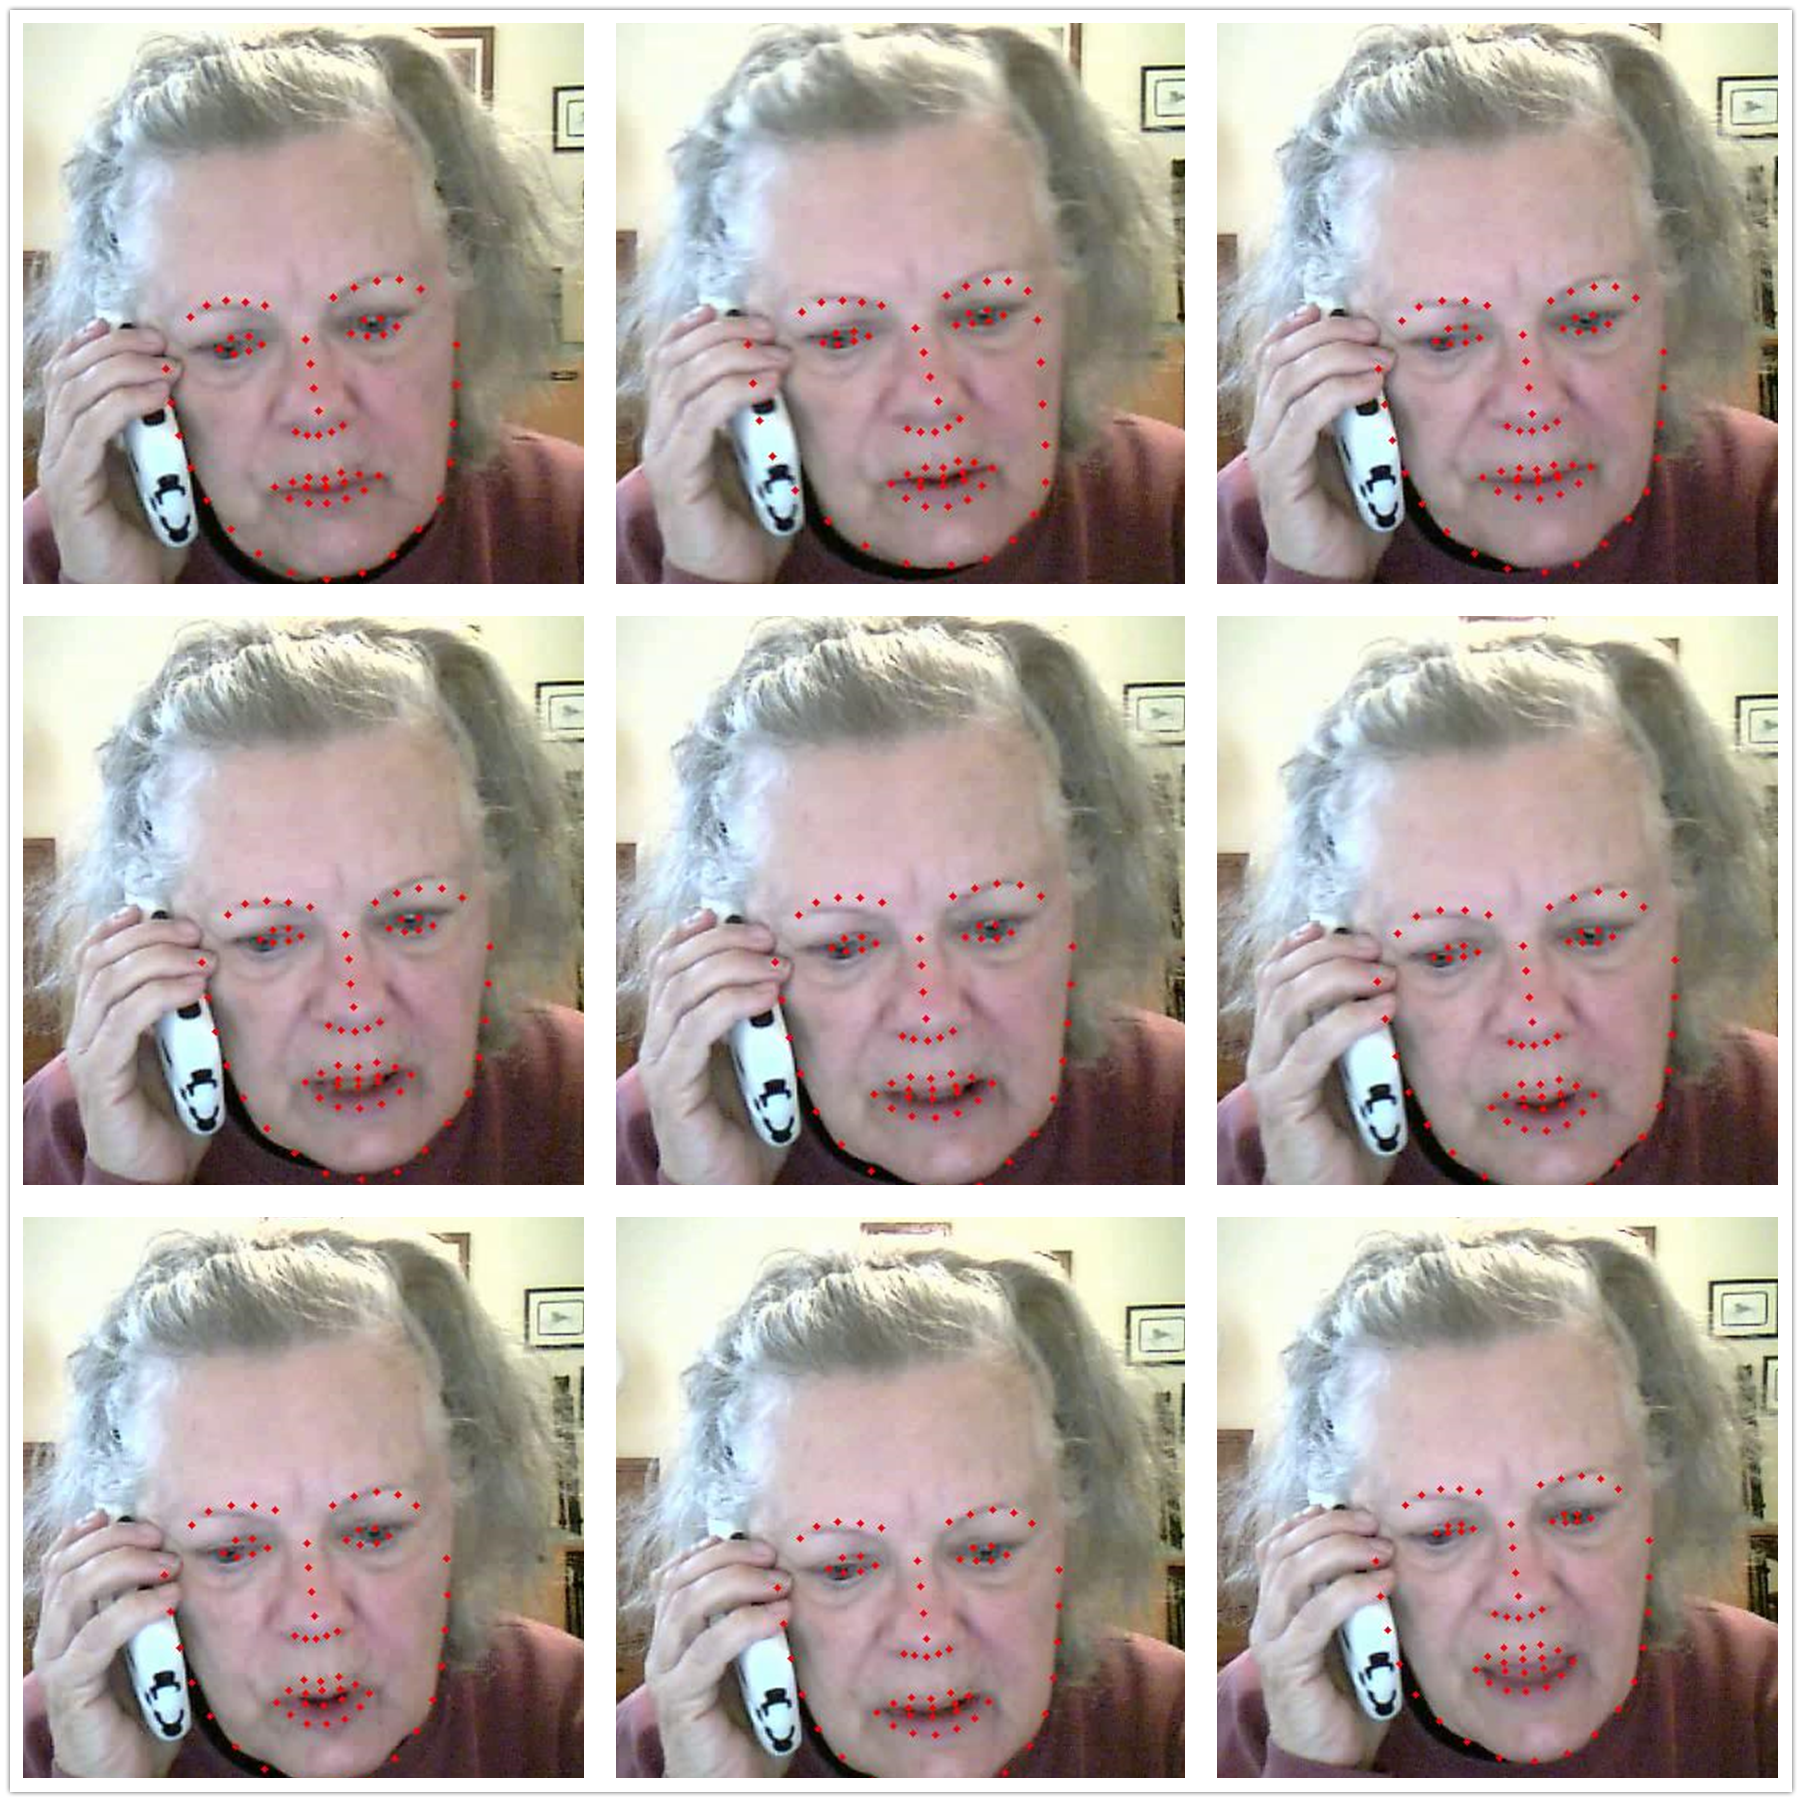
\includegraphics[width=100mm]{imgs/Talking_DRMF_140711_176_184.png}
\caption{Talking sequence tracked by DRMF}
\label{fig:DTS}
\end{figure}
\newpage
\subsection{Comparison}
The following are some examples for comparing two trackers. There are two version of DRMF tracker one is implemented by CUDA language the other is by C language. Although the C version of DRMF is very slow and very easy to run out of memory, the version implementd by CUDA is very fast as CUDA is using parallel computing. However, DRMF is not as accurate as Intraface and not suitable for this project. In many situations, DRMF try to fit a face and the fitting result is awful. The images with red points are tracked by Intraface, and the images with blue points is tracked by DRMF.
\newline
From figure above, it seems both tracker can only be used to trak one face at one time. DRMF detect the smaller face instead of the bigger one is possiblly because of the algorithm. The second and third frames are tracked by DRMF is not very accurate on the nose area. As the track point of mouth, intraface is better than DRMF.
In some frame, partial of face is out of frame. Intraface is better dealing with this type of situation. Intraface ignore those points that out of the images. DRMF tries to fit a face forcibly. It often lead to bad influence on the traking result shown in the figure.
\begin{figure}[p]
\centering

\includegraphics[width=110mm]{imgs/Tracking_Intraface_DRMF_compare_00.png}
\caption{Tracking result, red points tracked by Intraface and blue points tracked by DRMF}
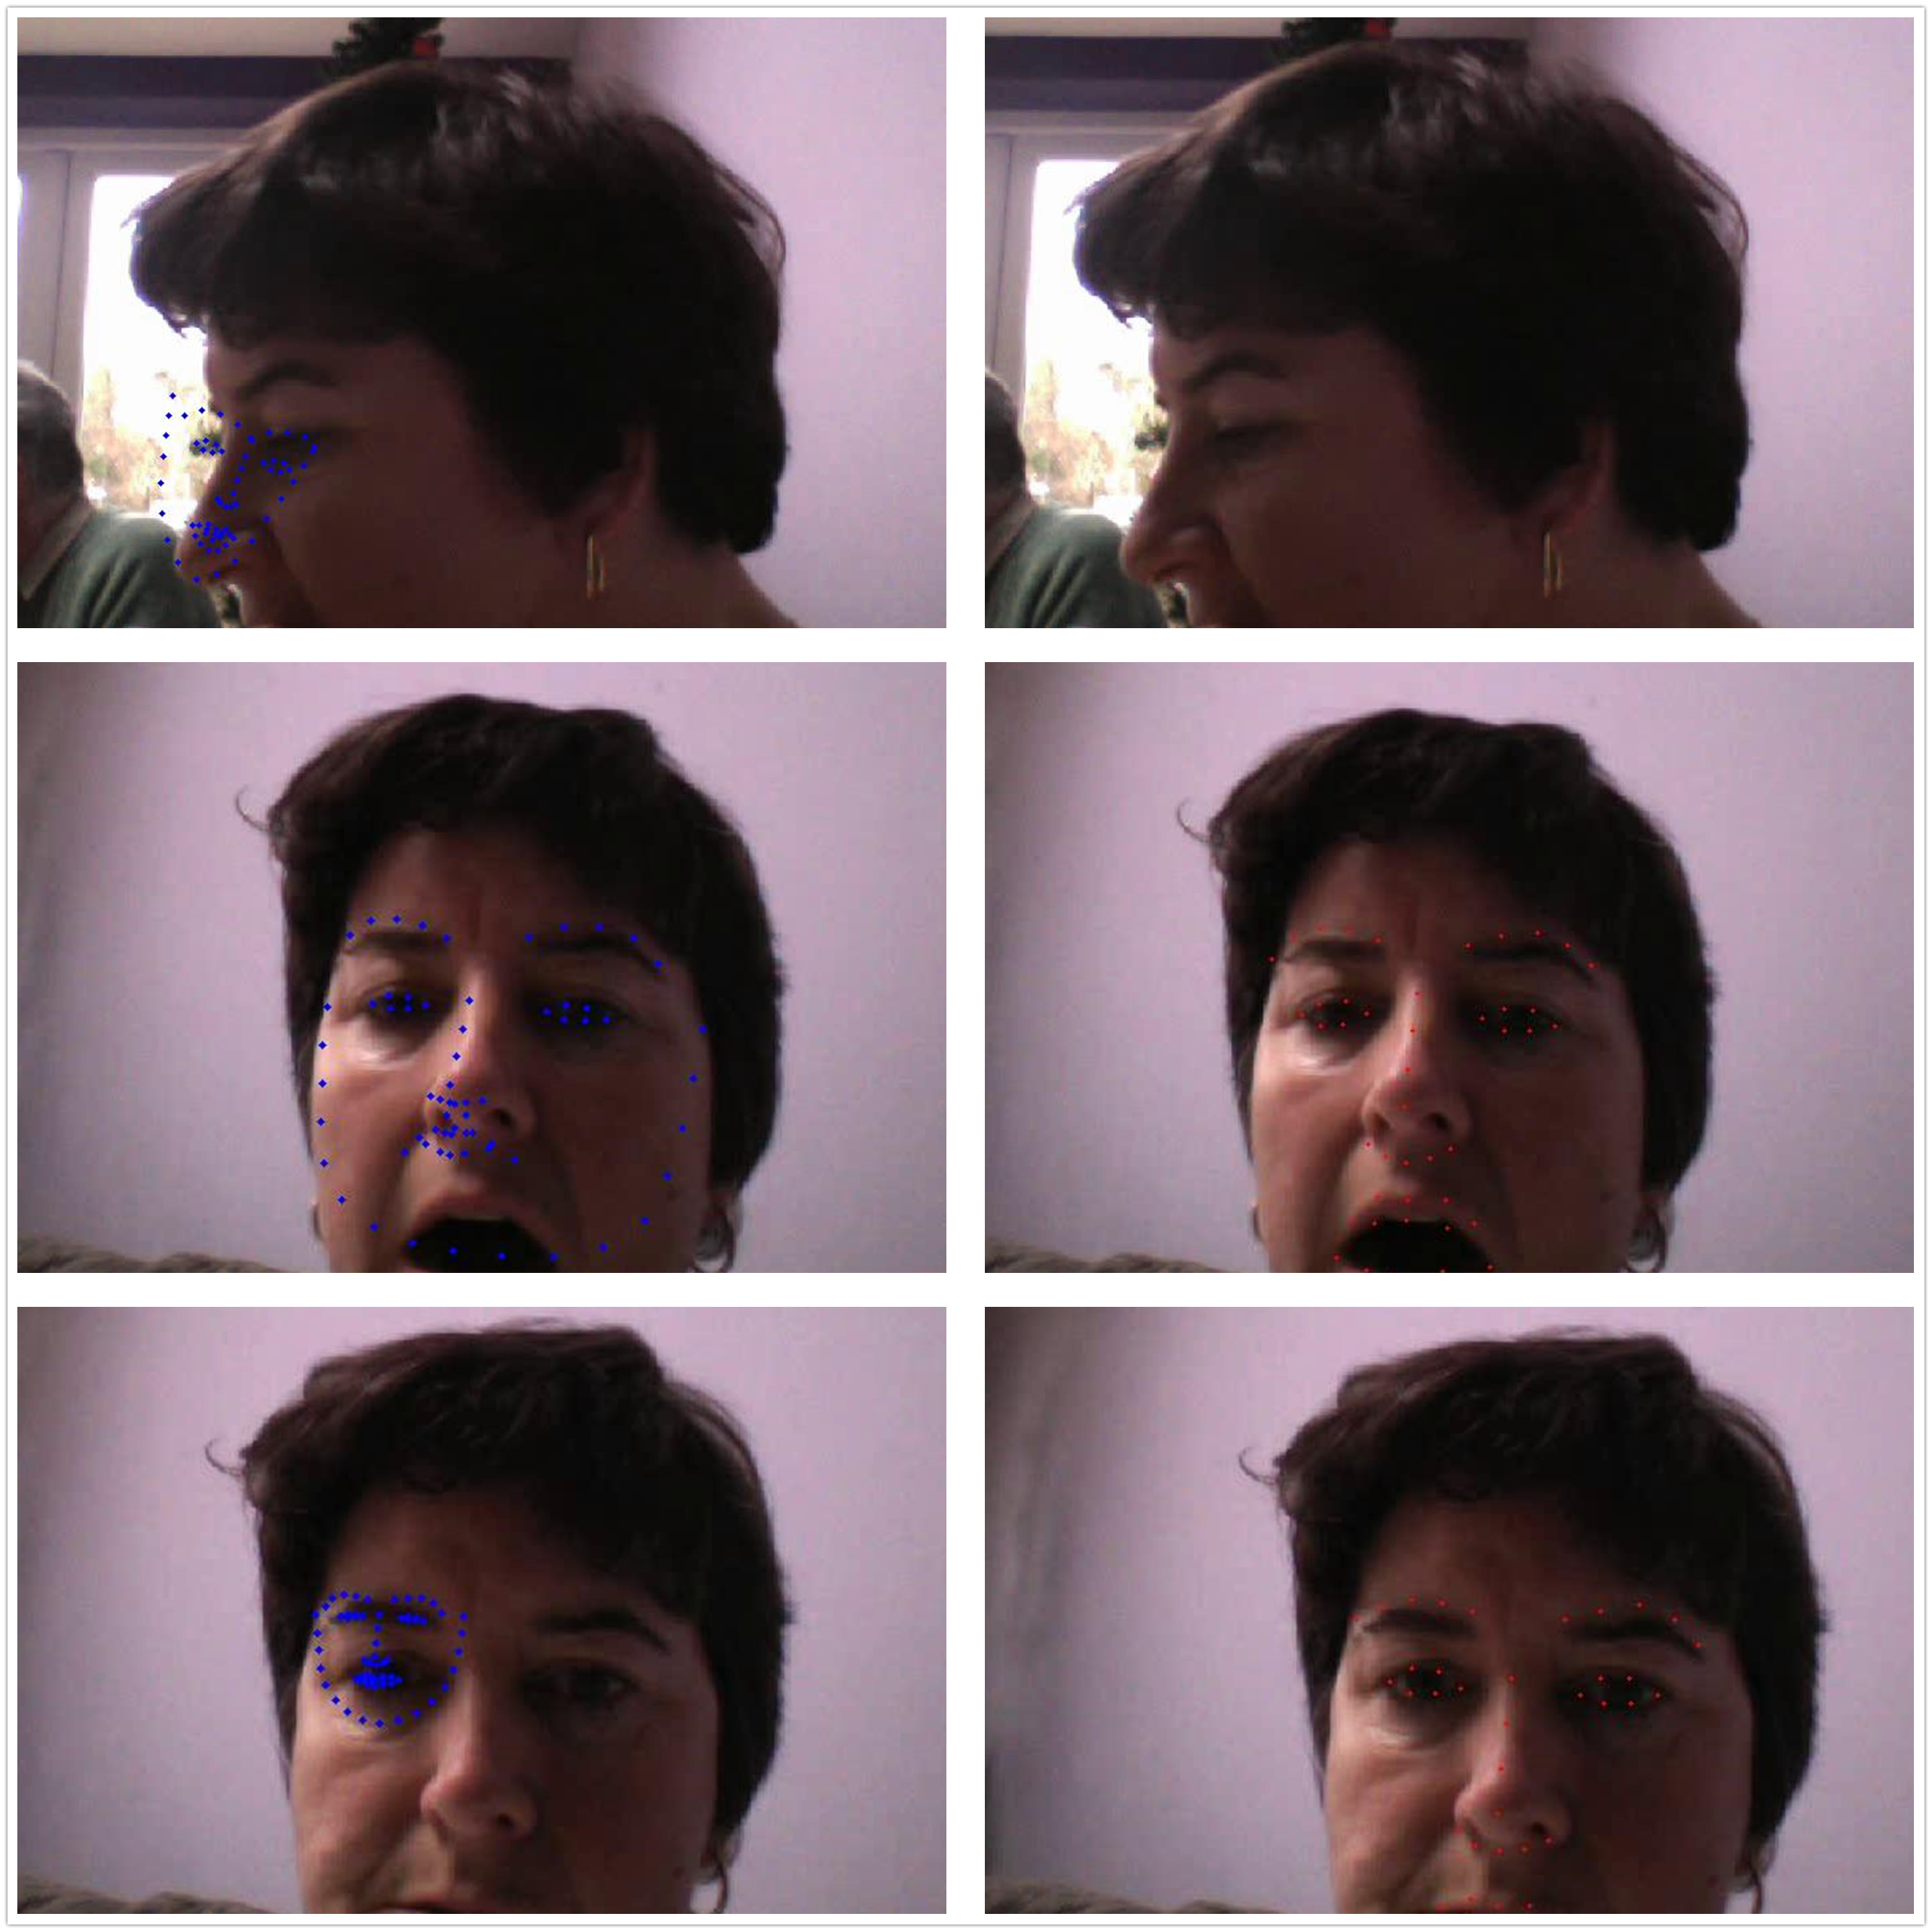
\includegraphics[width=110mm]{imgs/Tracking_Intraface_DRMF_comparison.png}
\caption{Tracking result, red points tracked by Intraface and blue points tracked by DRMF}
\end{figure}
\newpage
\section{Remove Head-pose}
The algroithm of removing head-pose from tracking points is in \cite{saragih2011deformable}. The following are some example of orginal track points and deformed points. Remove head pose of face and the warp the face to frontal direction is the most important part of extracting appearance feature. Here are two examples, from example one, rotation on x-y direction is mostly removed. In example two, the algorithm also show some efficient on remove head-pose of x-z direction and y-z direction.
\begin{figure}[ht]
\centering
\includegraphics[width=150mm]{imgs/160954_Deform_213.png}
\caption{Traking points and Deformed Points, Example 1}
\includegraphics[width=150mm]{imgs/160954_Deform_233.png}
\caption{Traking points and Deformed Points, Example 2}
\end{figure}
\newpage
\section{Warping}
In order to have the appearance image of the face after removed head-pose, it is necessary to warp the face with head pose. Basic idea is to for each triangles builded by shape points, the image points in the triagnles are projected to the corresponding triagnles built by deformed points. The following are some examples of face before and after warping:

\begin{figure}[ht]
\centering
\includegraphics[width=90mm]{imgs/Warping_Intraface_213.png}
\caption{Talking sequence tracked by DRMF}
\end{figure}
\newpage
\section{Feature Extraction}
The image after warping is not directly used for classfication, image feature are stelected to represent the image. Points, edges, ojects and texture are important features of an image. In this project, Local Binary Pattern are used for calssification as it's a very powerful feature for texuture classfication. 
\subsection{Local Binary Pattern}
LBP is chosen to be the feature for representing region of interest. \cite{shan2009facial} obtained best recognition result by using Support Vector Machine with Boosted-LBP features. Moreover, \cite{shan2009facial} shows LBP features perform stably and robustly on low-resolution face images. In the beginning, LBP was used for texture analysis, it has natural advantage on computational simplicity and ignoring illumination changes.
\newpage
\section{Postprocessing}
As it is known large margin classifiers are sensitive to the way features are scaled, it's better to normalize either the data or the kernal function \cite{ben2010user}. Feature of a image is represented by a vector, the number in the vector would influence the weight of feature in this dimension. As I would like to treat each dimension similar, I scale the number in the range of $[0,1]$.
\paragraph{Normalization}
The perfromance of SVM is usually better if the data is normalized. There are two ways of applying normalization, standardlizing the input features or normalizing the kernal function. As I am using the builtin function of libsvm \cite{CC01a}, so I standardlising the input features by substracting its mean and divide by its standard deviation.
\paragraph{Scaling}
The range of appearance feature vector and shape feature vector is different. I would like to treat then as the same. So I scale all the vector into the range of $[0, 1]$, by substract the minmun and divide by the maximum number of each dimension.